% !TEX encoding = UTF-8 Unicode
%!TEX root = ../Main/thesis.tex
% !TEX spellcheck = en-US
%%=========================================
\documentclass[../Main/thesis.tex]{subfiles}
\begin{document}
\chapter{Second Iteration  - First prototype}
\label{ch:development-1}
This chapter describes the second iteration of the development.
In this iteration a prototype of both the Android application and the back-end was developed.
The iteration ended with a demonstration and test of the prototypes for Øygarden Fire and Rescue.

\section{Android application}
The goal for this iteration was to implement the Bluetooth data collecting functionality, and the possibility to upload a completed session to the server, using the design proposed in Chapter~\ref{ch:requirements}.

This version of the app is shown in Figure~\ref{fig:app-first-prototype}.
The first screen in the application (see Figure~\ref{fig:app-first-prototype-sessionlist}) contains a list of available sessions. 
Each session is represented with a name and the name of the person who is supposed to use that session.
When a smoke diver is getting ready for the exercise he chooses the appropriate session from the list which takes him to the next screen.

The second screen in the app (see Figure~\ref{fig:app-first-prototype-trackingactivity}) tells the user that the app is not currently tracking and has a blue play-button and instructions telling the user to press the button to start the tracking.
When a user press the play-button a dialog-box is shown asking for confirmation that the user want to start the tracking. 
If the user confirms he is taken to the third screen (see Figure~\ref{fig:app-first-prototype-tracking}) and the app start searching for BLE-signals.
Every time the app receives a BLE-signal it stores the signal-strength, identifiers of the beacon transmitting the signal, data from the gyroscope and accelerometer in the phone, and a timestamp, as a datapoint in the current session.
When the user has finished the tracking and presses the stop-button a new dialog appears to confirm that the user want to end the tracking.
If the user confirms all the recorded data is uploaded to the server for processing, and a upload-dialog is shown (see Figure~\ref{fig:app-first-prototype-upload}.
After the uploading is finished the user is taken back to the list of available sessions.

\begin{figure}[h]
	\centering
	\begin{subfigure}{0.2\textwidth}
		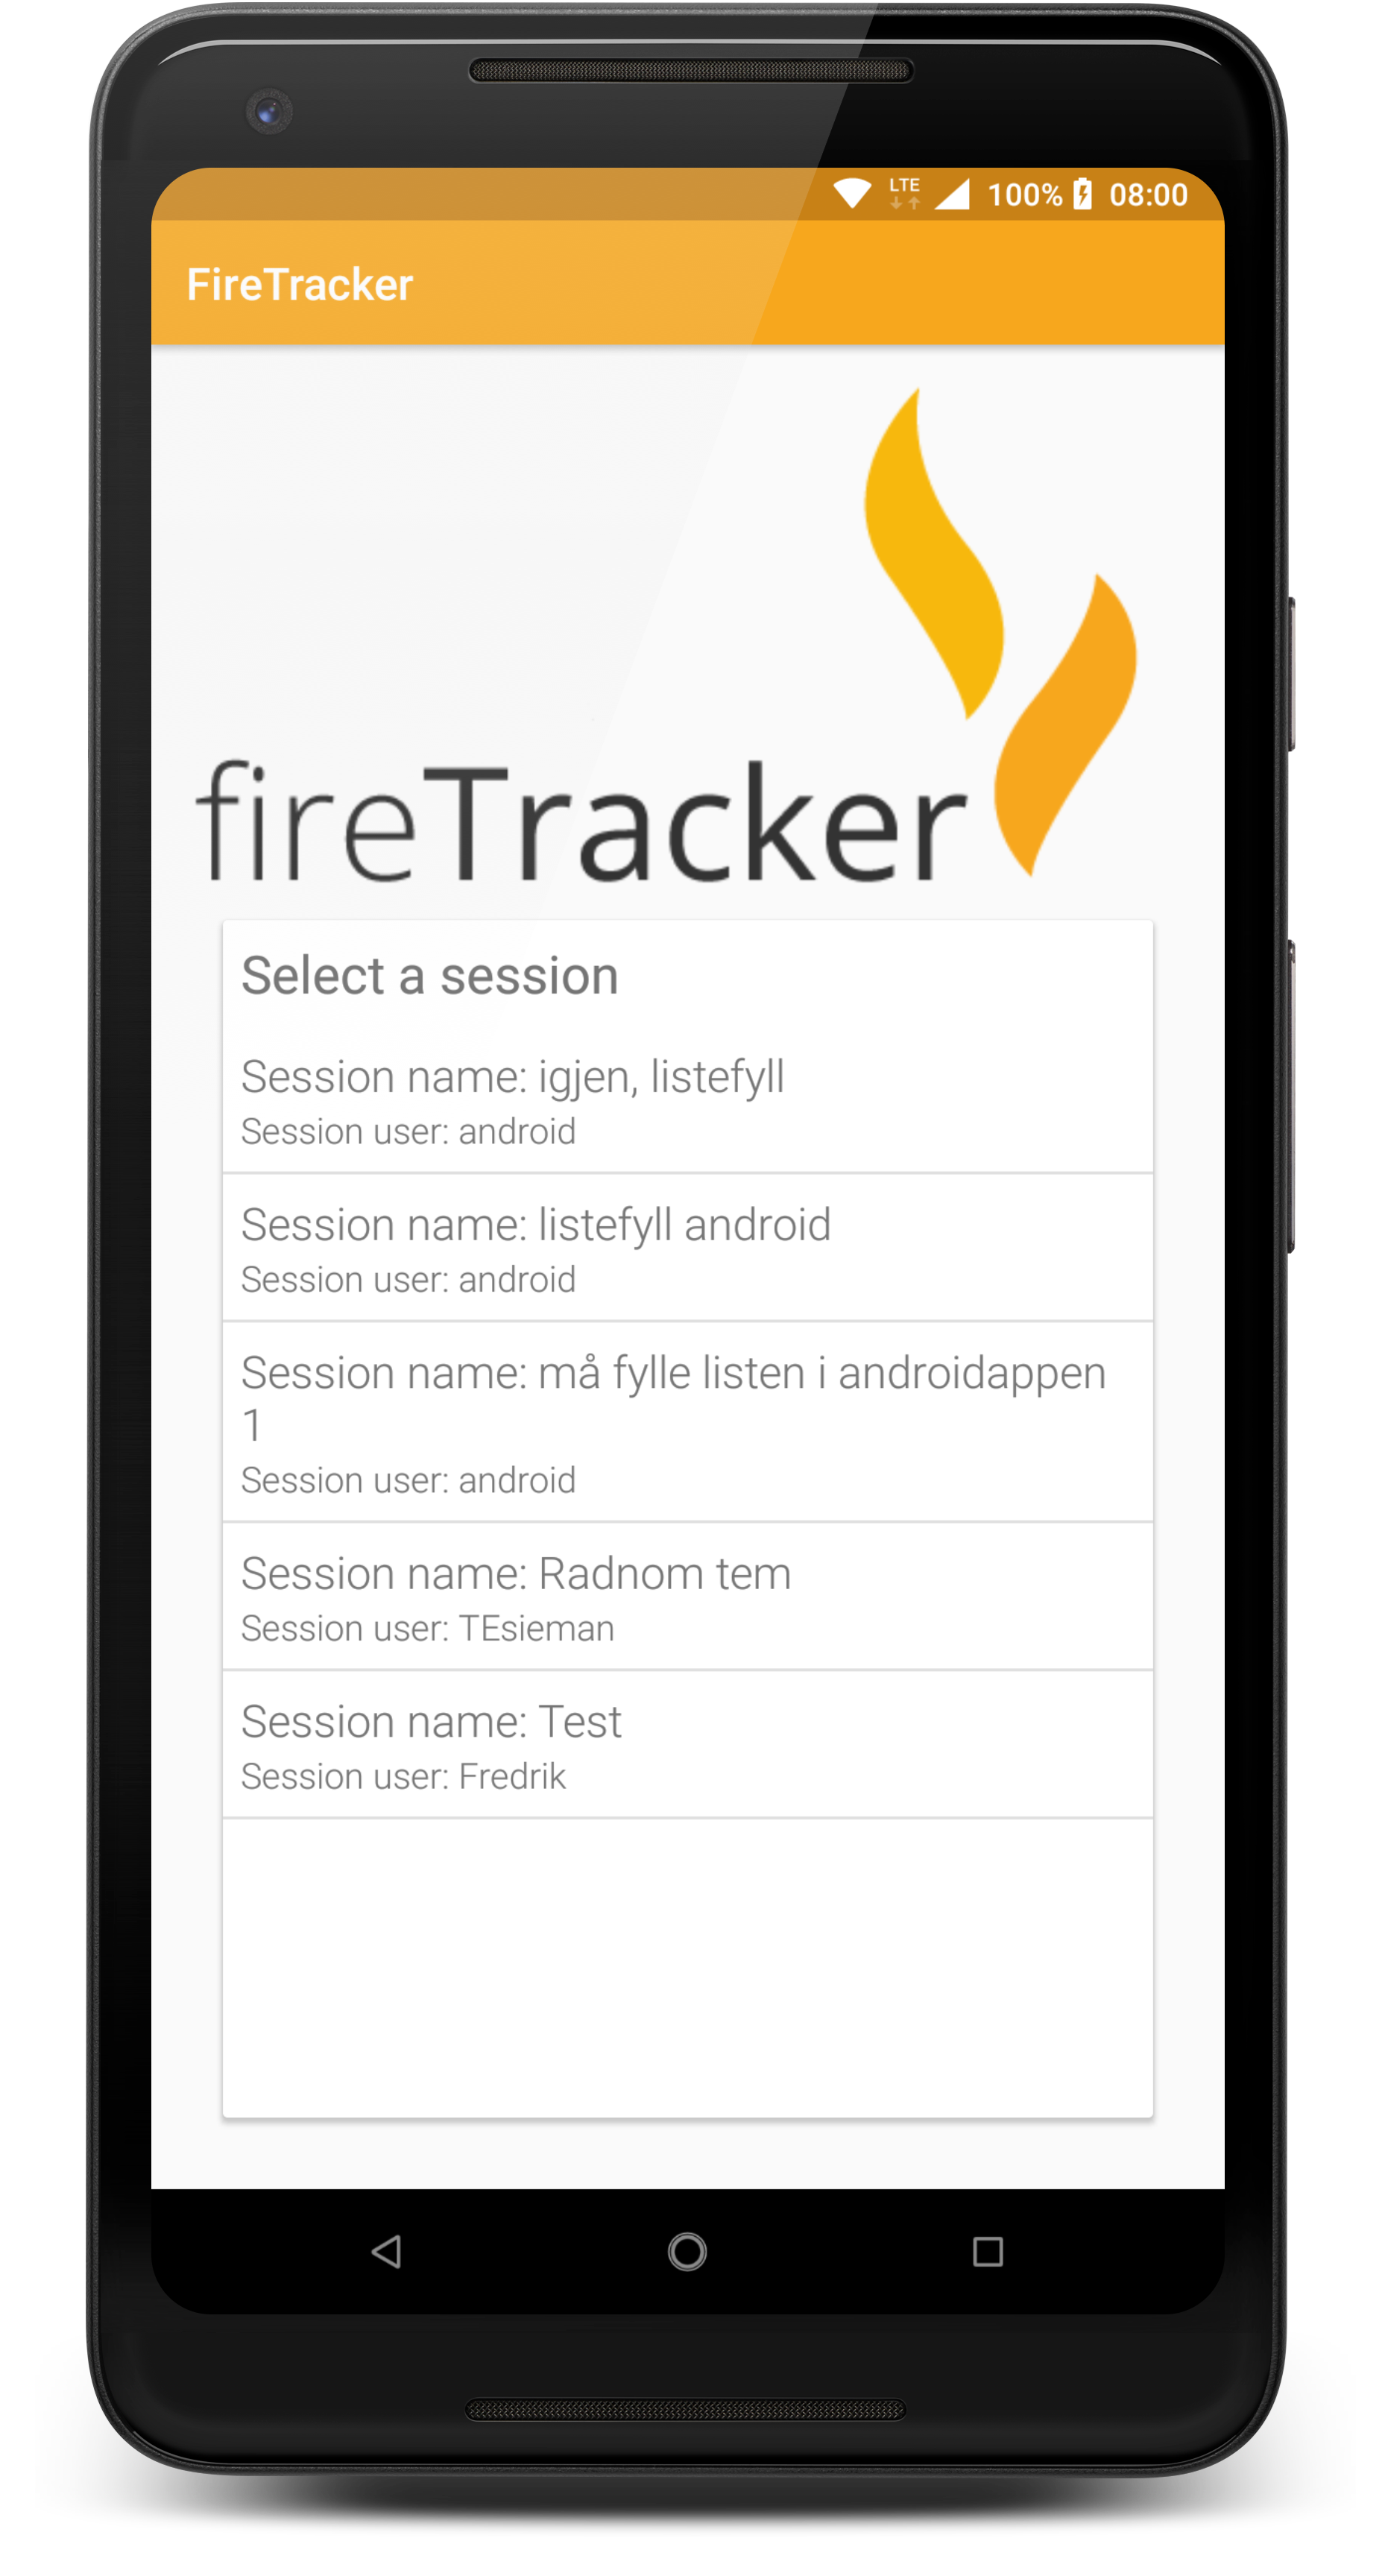
\includegraphics[width=\textwidth]{../fig/firetracker_app_old_1}
		\caption{List of sessions}
		\label{fig:app-first-prototype-sessionlist}
	\end{subfigure}
	\begin{subfigure}{0.2\textwidth}
		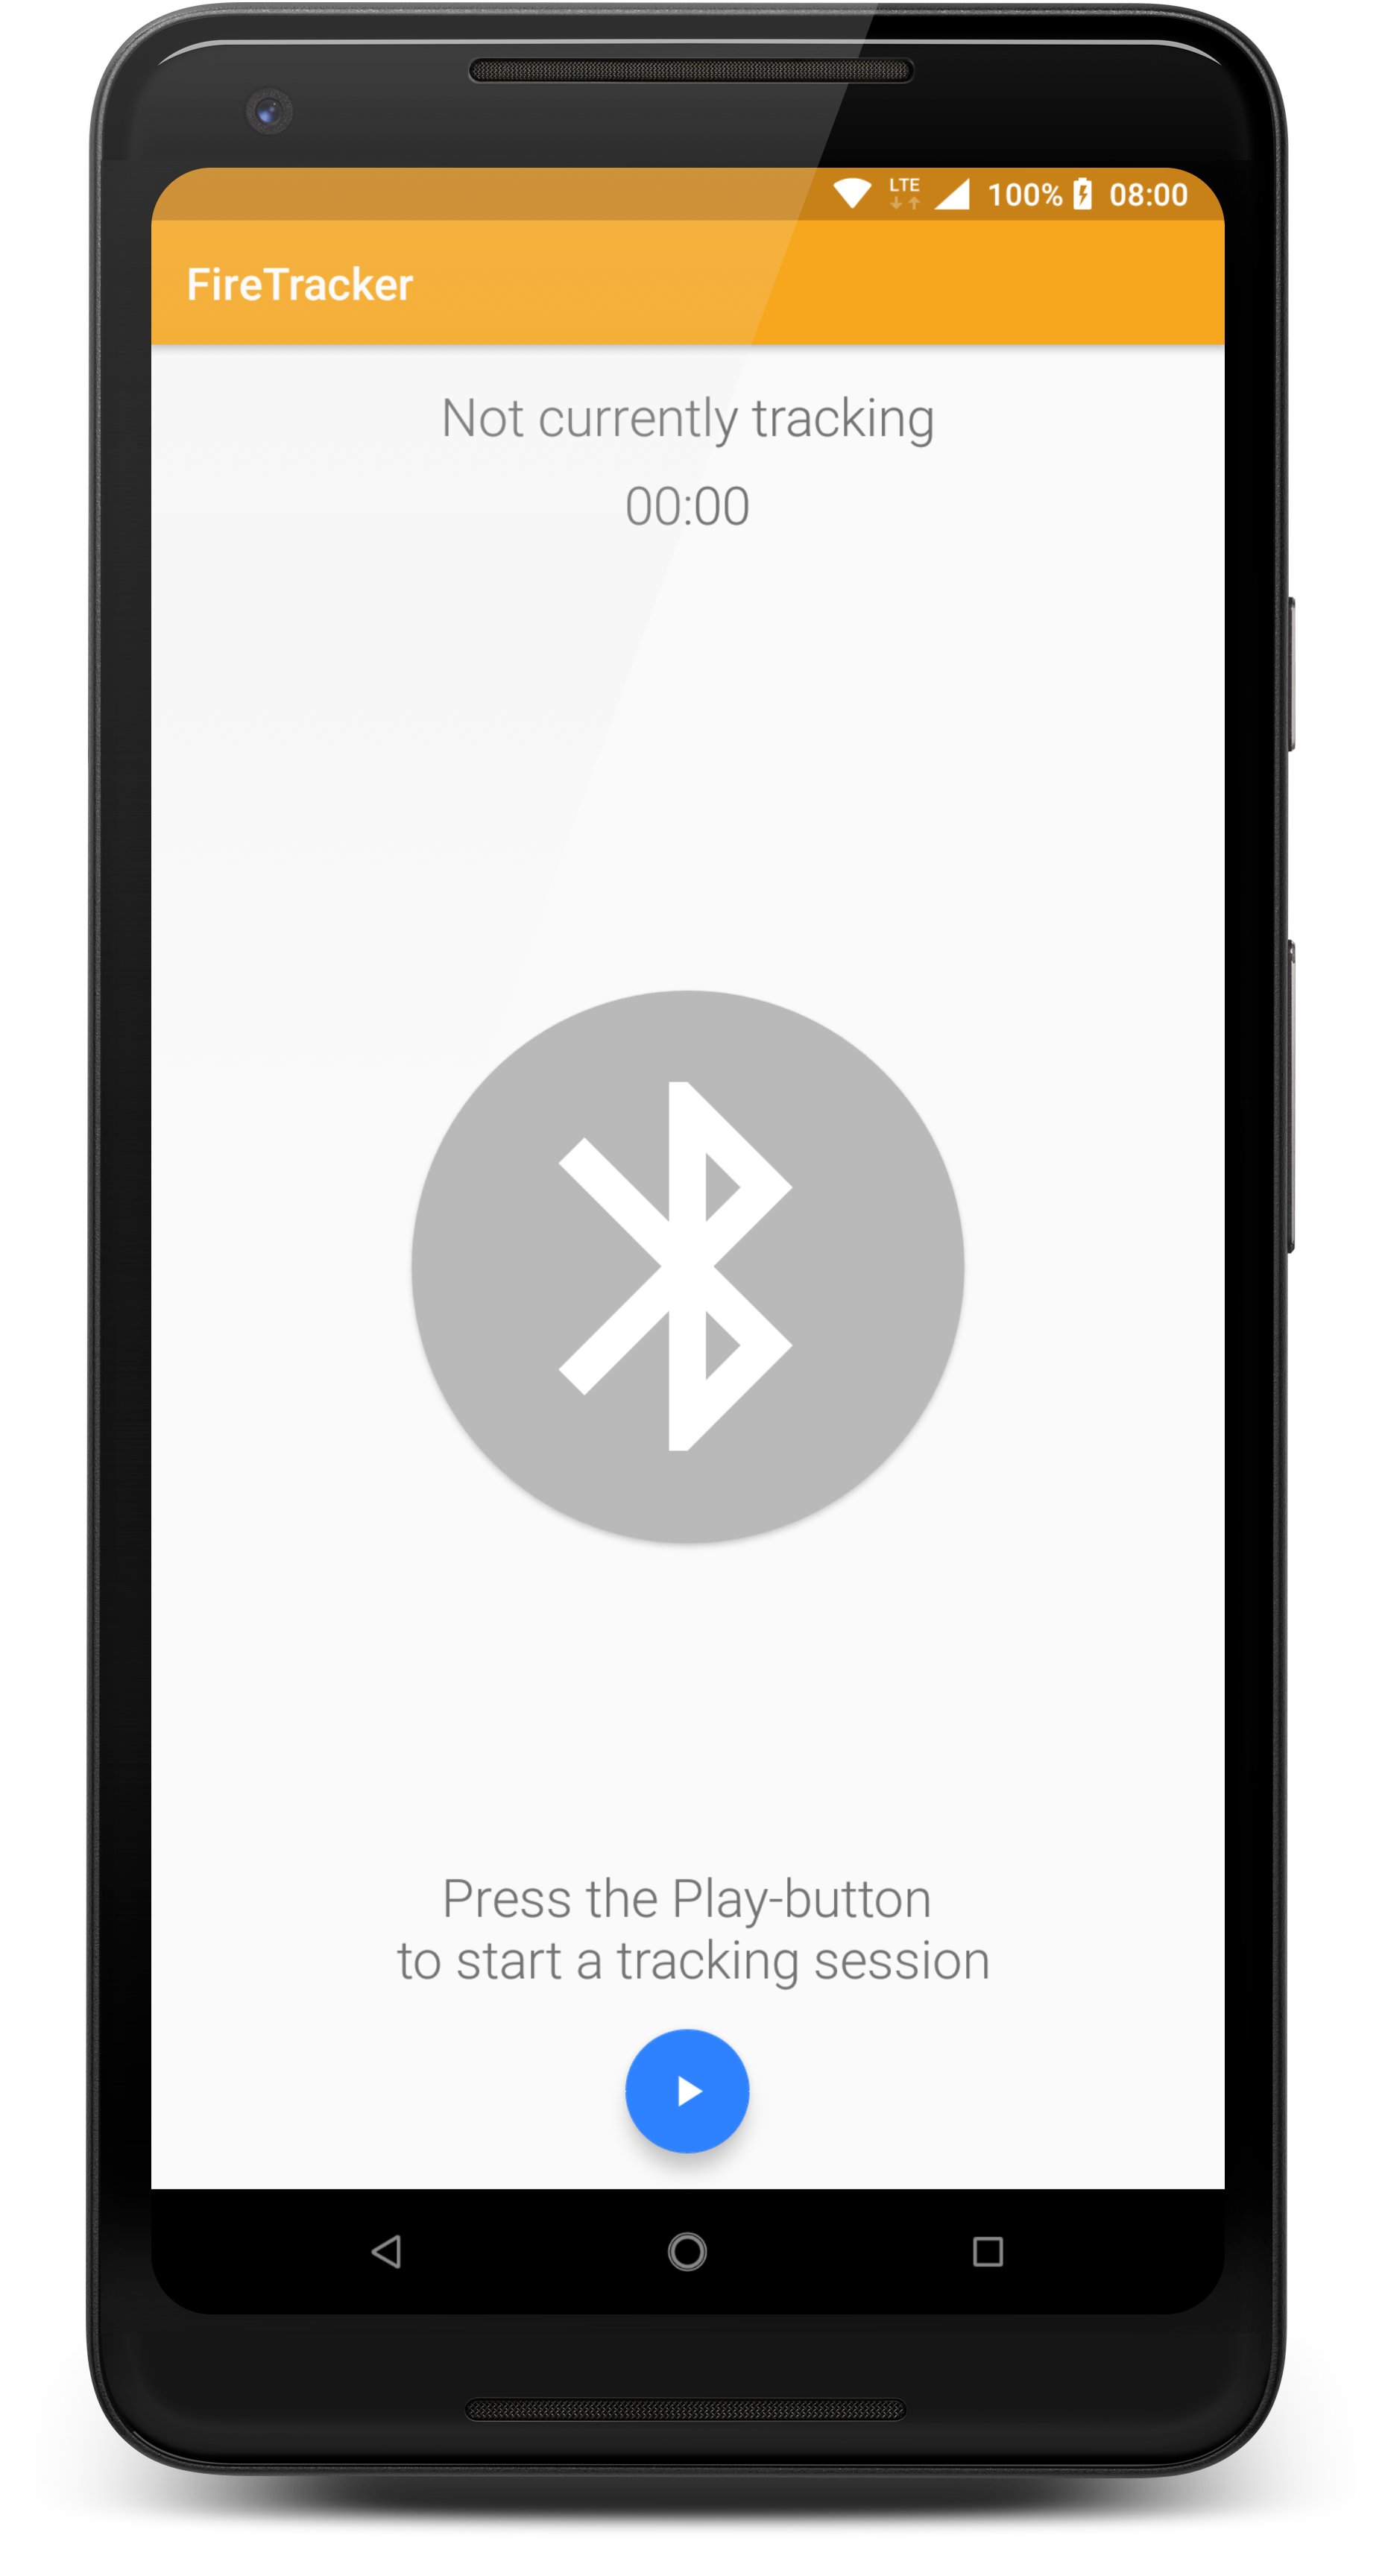
\includegraphics[width=\textwidth]{../fig/firetracker_app_old_2}
		\caption{Tracking activity}
		\label{fig:app-first-prototype-trackingactivity}
	\end{subfigure}
	\begin{subfigure}{0.2\textwidth}
		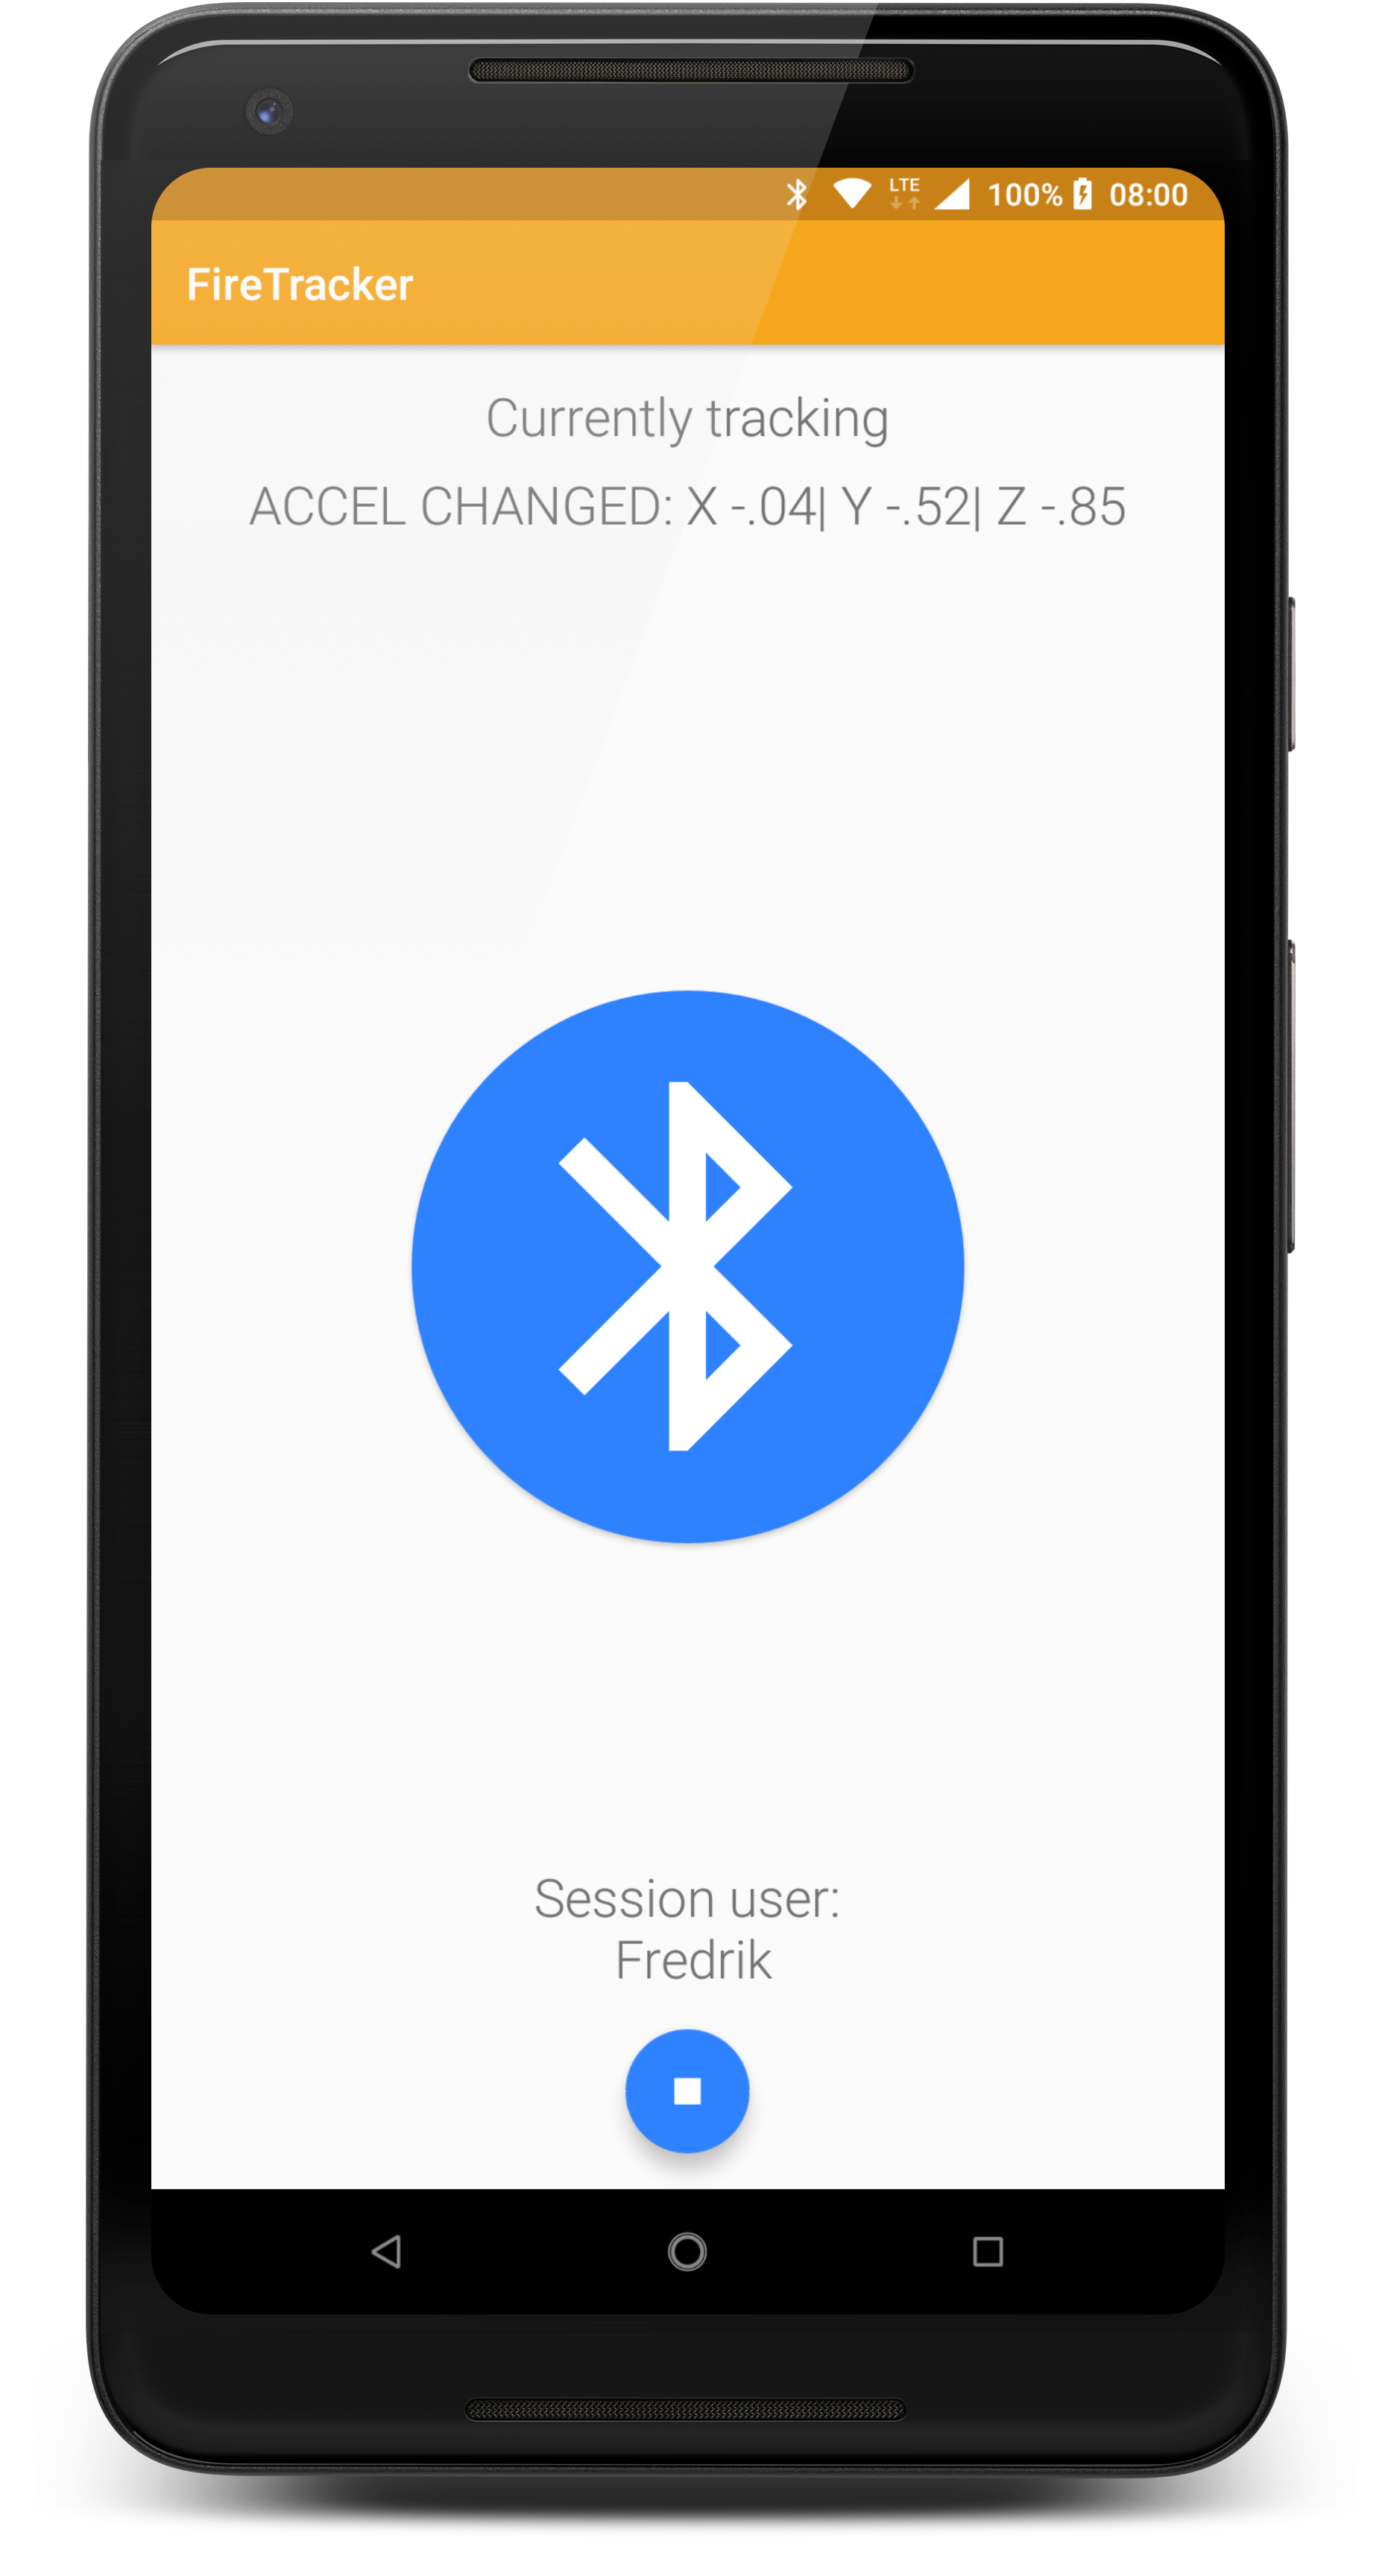
\includegraphics[width=\textwidth]{../fig/firetracker_app_old_3}
		\caption{Active tracking}
		\label{fig:app-first-prototype-tracking}
	\end{subfigure}
	\begin{subfigure}{0.2\textwidth}
		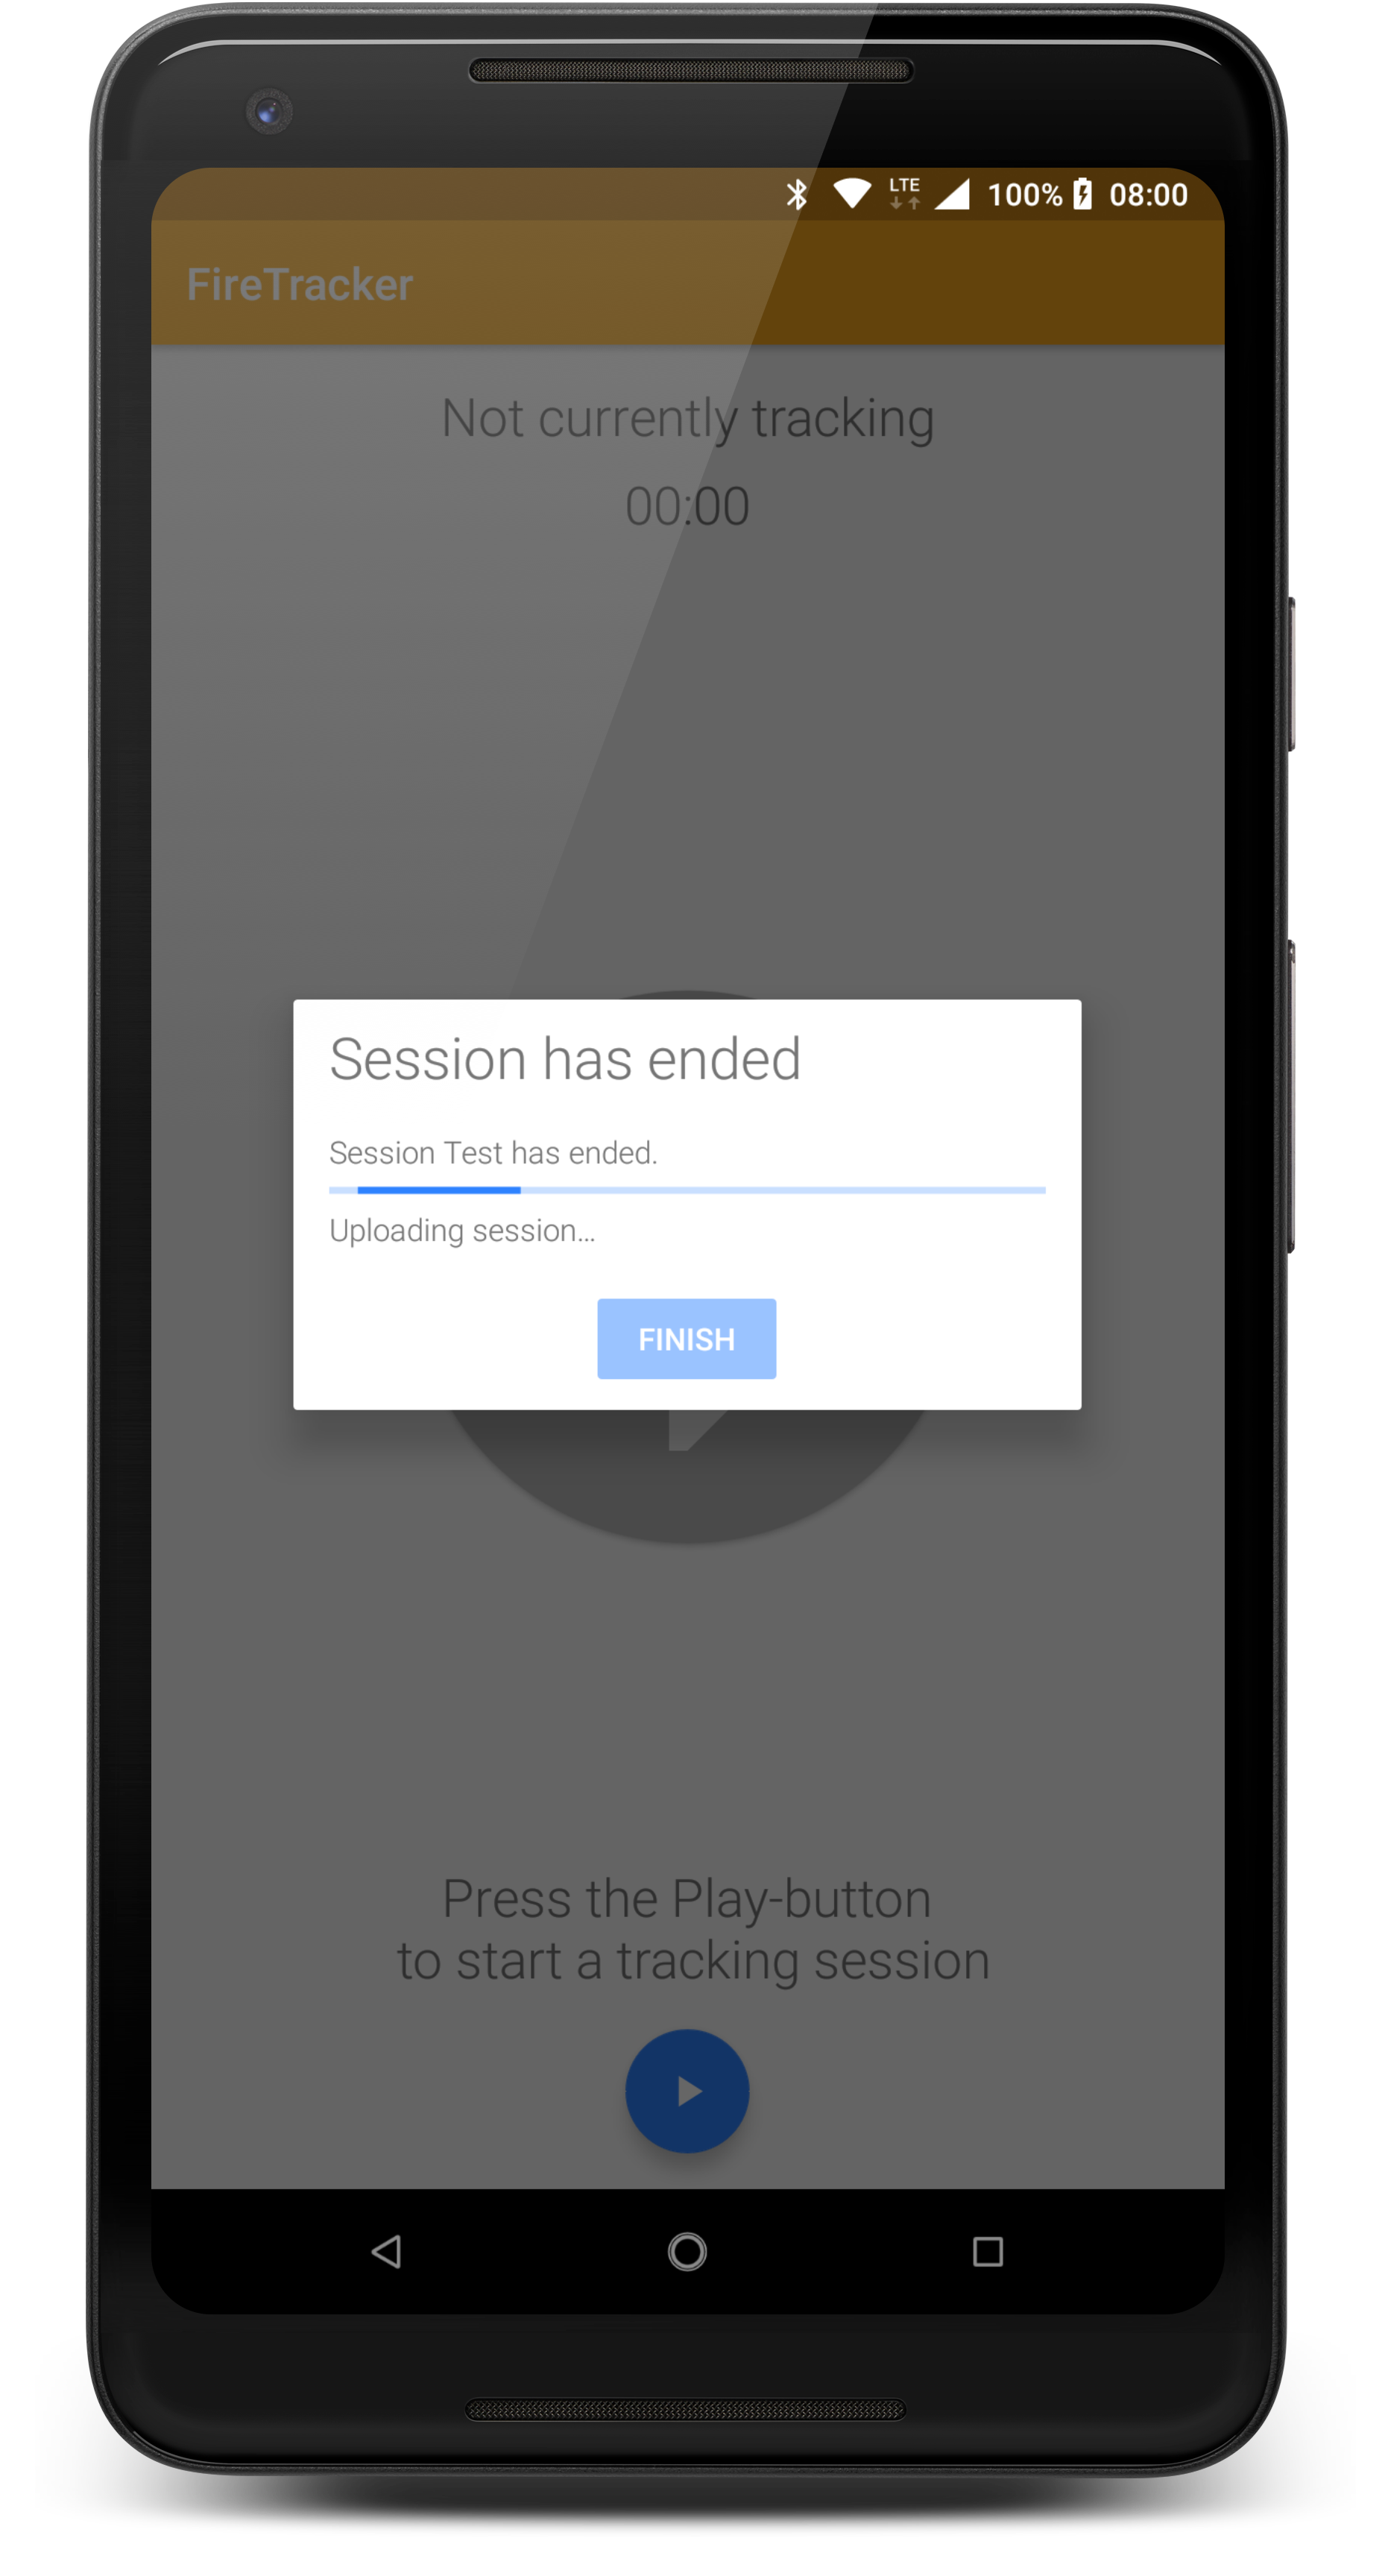
\includegraphics[width=\textwidth]{../fig/firetracker_app_old_4}
		\caption{Uploading data}
		\label{fig:app-first-prototype-upload}
	\end{subfigure}
	\caption{Screenshots of the Android application}
	\label{fig:app-first-prototype}
\end{figure}

\subsection*{Use of sensors}
In addition to tracking Bluetooth-data the app also records data from the built-in accelerometer and gyroscope in the smartphone.
The accelerometer was used to detect movement and create an estimate of how many steps the user takes during the tracking.
This information was then used to determine if the smoke diver was walking around or standing still within a location.

The gyroscope was used to collect information about the relative orientation of the smartphone. 
The intention was to use this data to determine the orientation of the smoke diver within the building, but it turned out that different devices had different zero positioning.
Therefore it was not possible to determine a consistent orientation across devices.
Instead the difference of orientation over a time interval was used to determine if the user rotating the device, and thereby rotating their head as the device. 

\section{Back-end}
The back-end of the FireTracker system consists of two parts.
A web-server that handles requests from the Android application and the exercise management tools and returns data to them
A part that processes the raw data from the Android app and outputs data about the locations and movements of the firefighters that can be used by the exercise management tool to create a visualization.
In this iteration the web-server functionality was implemented together with a basic processing algorithm.

\subsection{Web server}

\subsection{Data processing}

\section{Data Specifications}
\subsection{Session}
\begin{listing}[h]
	\begin{minted}
	[
	frame=lines,
	linenos
	]{json}
{
	"ID": <integer>,
	"Name": <string>,
	"User": <string>,
	"StartTime": <integer>,
	"EndTime": <integer>,
	"Datapoints": [<datapoint>],
	"Beacons": [<beacon>],
	"Locations": [<location>],
	"Finished": <boolean>,
	"Map": <string>
}
\end{minted}
\caption{Session data specification}
\label{listing:session-json-1}
\end{listing}

\subsection{Datapoint}
\begin{listing}[h]
	\begin{minted}
	[
	frame=lines,
	linenos
	]{json}
{
	"ID": <integer>,
	"SessionId": <integer>,
	"UUID": <string>,
	"Major": <string>,
	"Minor": <string>,
	"Timestamp": <integer>,
	"RSSI": <integer>,
	"Steps": <integer>,
	"RotationX": <float>,
	"RotationY": <float>,
	"RotationZ": <float>
}
\end{minted}
\caption{Datapoint data specification}
\label{listing:datapoint-json-1}
\end{listing}

\subsection{Beacon}
\begin{listing}[h]
	\begin{minted}
	[
	frame=lines,
	linenos
	]{json}
{
	"ID": <integer>
	"SessionId": <integer>
	"UUID": <string>,
	"Major": <string>,
	"Minor": <string>,
	"Name": <string>,
	"XCoordinate": <float>,
	"YCoordinate": <float>
}
\end{minted}
\caption{Beacon data specification}
\label{listing:beacon-json-1}
\end{listing}
\subsection{Location}

\begin{listing}[h]
	\begin{minted}
	[
	frame=lines,
	linenos
	]{json}
{
	"ID": <integer>,
	"SessionId": <integer>,
	"XCoordinate": <float>,
	"YCoordinate": <float>,
	"Duration": <integer>,
	"Walking": <boolean>,
	"HeadMovement": <boolean>
}
\end{minted}
\caption{Location data specification}
\label{listing:location-json-1}
\end{listing}

\section{Testing}
\subsection{Demonstration and testing}
\subsection{Feedback}

\end{document}
